\documentclass[10pt]{article}
 \usepackage{graphicx}
 \usepackage[tight]{subfigure}
 \usepackage{amssymb}
 \usepackage{mathtools}
 \usepackage{amsmath}
 \usepackage{clrscode}
 \usepackage{algorithmicx}
\usepackage{algorithm}
\usepackage[noend]{algpseudocode}
\usepackage{xcolor}
\usepackage{listings}
\usepackage{hyperref}
\usepackage{color}

\definecolor{dkgreen}{rgb}{0,0.6,0}
\definecolor{gray}{rgb}{0.5,0.5,0.5}
\definecolor{mauve}{rgb}{0.58,0,0.82}

\lstset{frame=tb,
  language=Python,
  aboveskip=3mm,
  belowskip=3mm,
  showstringspaces=false,
  columns=flexible,
  basicstyle={\small\ttfamily},
  numbers=none,
  numberstyle=\tiny\color{gray},
  keywordstyle=\color{blue},
  commentstyle=\color{dkgreen},
  stringstyle=\color{mauve},
  breaklines=true,
  breakatwhitespace=true,
  tabsize=3
}
\hypersetup{
    colorlinks=true,
    linkcolor=blue,
    filecolor=magenta,      
    urlcolor=cyan,
    pdftitle={Overleaf Example},
    pdfpagemode=FullScreen,
    }

\urlstyle{same}


\algrenewcommand{\algorithmiccomment}[1]{ \{ #1 \} }

\newif\ifboldnumber
\newcommand{\boldnext}{\global\boldnumbertrue}

 \setlength{\oddsidemargin} {0 in}
\setlength{\textwidth} {6.5 in}
\setlength{\textheight} {8.5 in}
\setlength{\topmargin} {-0.5 in}
\def\h{\hspace{-.9pt}{\_}}
\newcommand{\reminder}[1]{ [[[ \marginpar{\mbox{$<==$}} #1 ]]] }
\newcommand{\eatreminders}[0]{\renewcommand{\reminder}[1]{}}
\newcommand\quoted[1]{``#1''}
\author{Brian Zhu\\
\url{https://github.com/zhubiii/CSE360} }
\date{}
\title{CSE 360: Workshop 1\\
}
\begin{document}

\maketitle
 
\begin{enumerate}
    \item
    \begin{itemize}
        \item This code can be done by first finding the parameterization of an ellipse.
        \item $x=acos(t)$ $y=bsin(t)$
        \item We then define our 2D rotation matrix as: $\begin{bmatrix}
            cos(\theta) & -sin(\theta) \\
            sin(\theta) & cos(\theta)
        \end{bmatrix}$ with our desired $\theta$ being $\pi / 6 = 30deg$
        \item $\begin{bmatrix}
            cos(\theta) & -sin(\theta) \\
            sin(\theta) & cos(\theta)
        \end{bmatrix} \begin{bmatrix}
            acos(t) \\
            bsin(t)
        \end{bmatrix}$
        \item We simply multiply the parameterization as a vector with the rotation matrix and we get the result below
        \item $x=cos(\theta)acos(t) - sin(\theta)bsin(t)$
        \item $y=sin(\theta)acos(t) + cos(\theta)bsin(t)$
        \item We must then take the derivative of both x and y such that we can give it to our controller
        \item $x'=ux=-acos(\theta)sin(t) - bsin(\theta)cos(t)$
        \item $y'=uy=bcos(\theta)cos(t) - asin(\theta)sin(t)$
        \begin{lstlisting}
        ### Problem 1
        t = t+5*pi/4 
        des_theta = pi/6 #30 degrees
        a = 4
        b = 2
        rot_matrix = np.array([[cos(des_theta), -sin(des_theta)],[sin(des_theta), cos(des_theta)]])
        vec_ctrl = np.array([[a*cos(t)],[b*sin(t)]])
        res = np.matmul(rot_matrix,vec_ctrl)
        x = res[0][0]
        y = res[1][0]
        ux = -a*cos(des_theta)*sin(t) - (b*sin(des_theta)*cos(t))
        uy = b*cos(des_theta)*cos(t) - (a*sin(des_theta)*sin(t) 
        \end{lstlisting}
        \item The code above essentially does all of the steps just listed. We also offset the time so that it more closely matches the coordinates of the picture
        \item \url{https://colab.research.google.com/drive/1EaDW4lujLjVALhCu_KfJYt0yln_QgOTa#scrollTo=U4ZDMbbzEXjI}
    \end{itemize}
    \item
    \begin{itemize}
        \item This code starts by converting the polar equation to parametric
        \item we start with the equation of $r=(sink\theta)+2$
        \item We then solve for $\theta$
        \item $r-2=sink\theta\implies\theta=arcsin(r-2)/k$
        \item Then we plug in $r$ back into that equation so that our final equation becomes:
        \item $\theta = \frac{arcsin(sin(kt)+2-2)}{k}=kt/k = t$
        \item We also know that to convert polar to parametric is the following two equations for x and y. So we substitute $r$ and $\theta$
        \item $x=rcos\theta = (sin(kt)+2)(cos(t))$
        \item $y=rsin\theta = (sin(kt)+2)(sin(t))$
        \item We must differentiate these to allow them to work in our controller as inputs
        \item $x'=ux=kcos(t)cos(kt) - (sin(t)(sin(kt)+2)$
        \item $y'=uy=cos(t)(sin(kt)+2)+(ksin(t)cos(kt))$
        \item The code below summarizes the above steps and we can follow each step of the process
        \item \begin{lstlisting}
        ### Problem 2
        k = 5   # number of pedals
        amplitude = 2  # how far the pedal extends
        theta = t+3*pi/2
        kt = k*theta
        r = sin(kt) + amplitude
        x = r*cos(theta)
        y = r*sin(theta)
        ux = (k*cos(theta)*cos(kt)) - (sin(theta)*(sin(kt)+amplitude))
        uy = cos(theta)*(sin(kt)+amplitude) + (k*sin(theta)*cos(kt))
        \end{lstlisting}
        \item Note that we also offset the theta by $3\pi/2$ so that it lines up with the coordinates of the given picture
        \item The next part of this question asks for a vertical wind and to compensate it using a PI controller
        \item \begin{lstlisting}
        vertical_wind = ([5,10]) #diagonal wind so that we can see the error more clearly

        # FOR PROBLEM 2
        x = simulate(dt, x, u+vertical_wind)
        \end{lstlisting}
        \item The code above is the code to add a wind. Next we must implement a PI controller
        \item \begin{lstlisting}
        # Note that p is our pose and err_dt is the accumulated error for the PI controller
        def control(t, p, err_dt): 
            k = 5   # number of pedals
            amplitude = 2  # how far the pedal extends
            theta = t+3*pi/2
            kt = k*theta
            r = sin(kt) + amplitude
            x = r*cos(theta) # tells us where we should be as a function of time
            y = r*sin(theta)
            #ux = (k*cos(theta)*cos(kt)) - (sin(theta)*(sin(kt)+amplitude))
            #uy = cos(theta)*(sin(kt)+amplitude) + (k*sin(theta)*cos(kt))
            
            # PI-Controller
            pk = 15                 # Proportional Constant            
            ik = .5                 # Integral Constant
            errx = x - p[0]         # To calculate our error, we use the x and y calculated in the first half of the code which tells us exactly where we should be as a function of time
            erry = y - p[1]
            err_dt[0] += errx
            err_dt[1] += erry
            ux = pk*(errx) + ik*(err_dt[0])
            uy = pk*(erry) + ik*(err_dt[1]) 
        \end{lstlisting}
        \item The code for this is located at the same place as the last problem, just remember to comment out the right things in the "Control Policy" and "Running the Simulator" block
        \item \url{https://colab.research.google.com/drive/1EaDW4lujLjVALhCu_KfJYt0yln_QgOTa#scrollTo=U4ZDMbbzEXjI}
    \end{itemize}
    \item
    \begin{itemize}
    \item This problem was relatively easy. We just needed to change the size of our vector space to be 3 instead of 2 and then use the right matplotlib functions
    \item \begin{lstlisting}
    x = array([0., 0., 0.]
    ax = plt.axes(projection='3d')
    ax.plot3D(x_log[:,0], x_log[:,1], x_log[:,2]
    # Path
    ax.plot3D(x_log[:,0], x_log[:,1], x_log[:,2], 'r--')
    
    # Initial conditions
    ax.scatter(x_log[t,0], x_log[t,1], x_log[t,2]
    \end{lstlisting}
    \item To get a helix we simply do a circle for x and y and then a constant speed for z
    \item \begin{lstlisting}
        ux = -sin(t)
        uy = cos(t)
        uz = t
    \end{lstlisting}
    \item 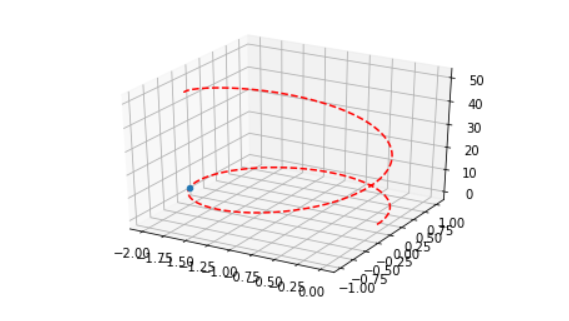
\includegraphics[scale=0.5]{3dHelix.png}
    \item The code for this is in a different colab linked below
    \item \url{https://colab.research.google.com/drive/1slAcQ8Ejpf-VyxE00SoextLREvKD_XoL#scrollTo=U4ZDMbbzEXjI}
    \end{itemize}
    \item
    \begin{itemize}
        \item Here we need to define our various waypoints that do not collide with the obstacles
        \item  $P = \{(-5,-7), (10,-7), (10,2.5), (0, 2.5), (0, 7), (3, 7), (3,0), (0,0), (0, 10), (9,10)\}$
        \item  $t_i = i$ for $i=1,...,10$
        \item With all of that defined, we simply plug in to the straight line trajectory equation for x and y for each time step such that we obtain a piecewise function
        \item $\gamma(t)=a_1t+a_0$
        \item where $a_1=\frac{p_f-p_0}{t_f} and a_0=p_0$
        \item  $\gamma(t) = 
        \begin{dcases}
            \gamma_{0,1}(t) =
             \begin{bmatrix}
                15t-5\\ -7
             \end{bmatrix}
             , & t\in [t_0, t_1] \\
            \gamma_{1,2}(t) =
             \begin{bmatrix}
                10\\ 9.5t-7
             \end{bmatrix}
             , & t\in [t_1, t_2] \\
            \gamma_{2,3}(t) =
             \begin{bmatrix}
                -10t+10\\ 2.5
             \end{bmatrix}
             , & t\in [t_2, t_3] \\
            \gamma_{3,4}(t) =
             \begin{bmatrix}
                0\\ 4.5t+2.5
             \end{bmatrix}
             , & t\in [t_3, t_4] \\
            \gamma_{4,5}(t) =
             \begin{bmatrix}
                -3t\\ 7
             \end{bmatrix}
             , & t\in [t_4, t_5] \\
            \gamma_{5,6}(t) =
             \begin{bmatrix}
                3\\ -7t+7
             \end{bmatrix}
             , & t\in [t_5, t_6] \\
            \gamma_{6,7}(t) =
             \begin{bmatrix}
                -3t+3\\ 0
             \end{bmatrix}
             , & t\in [t_6, t_7] \\
            \gamma_{7,8}(t) =
             \begin{bmatrix}
                0\\ 10t
             \end{bmatrix}
             , & t\in [t_7, t_8] \\
            \gamma_{8,9}(t) =
             \begin{bmatrix}
                9t\\ 10
             \end{bmatrix}
             , & t\in [t_8, t_9] \\
        \end{dcases} $
            
    \end{itemize}

    \item
    \begin{itemize}
        \item We reuse the same waypoints but now plug into the cubic polynomial trajectory
        \item See the code at \url{https://github.com/zhubiii/CSE360/blob/main/workshop1/calcCubic.py} for a script to calculate those coefficients
        \item  $P = \{(-5,-7), (10,-7), (10,2.5), (0, 2.5), (0, 7), (3, 7), (3,0), (0,0), (0, 10), (9,10)\}$
        \item $t(t) = [1,t,t^2,t^3]^\top$
        \item  $\gamma(t) = 
        \begin{dcases}
            \gamma_{0,1}(t) =
             \begin{bmatrix}
                [-5, 0, 43, -28]t(t)\\ [-7, 0, -2, 2]t(t)
             \end{bmatrix}
             , & t\in [t_0, t_1] \\
            \gamma_{1,2}(t) =
             \begin{bmatrix}
                [10, 2, -3, 1]t(t)\\ [-7, 2, 4.125, -1.375]t(t)
             \end{bmatrix}
             , & t\in [t_1, t_2] \\
            \gamma_{2,3}(t) =
             \begin{bmatrix}
                [10, 2, -5.33, 1.185]t(t)\\ [2.5, 2, -2, 0.444]t(t)
             \end{bmatrix}
             , & t\in [t_2, t_3] \\
            \gamma_{3,4}(t) =
             \begin{bmatrix}
                [0, 2, -1.5, 0.25]t(t)\\ [2.5, 2, -0.65, 0.109]t(t)
             \end{bmatrix}
             , & t\in [t_3, t_4] \\
            \gamma_{4,5}(t) =
             \begin{bmatrix}
                [0, 2, -.84, 0.112]t(t)\\ [7, 2, -1.2, 0.16]t(t)
             \end{bmatrix}
             , & t\in [t_4, t_5] \\
            \gamma_{5,6}(t) =
             \begin{bmatrix}
                [3, 2, -1, 0.11]t(t)\\ [7, 2, -1.58, 0.175]t(t)
             \end{bmatrix}
             , & t\in [t_5, t_6] \\
            \gamma_{6,7}(t) =
             \begin{bmatrix}
                [3, 2, -1.04, 0.09]t(t)\\ [0, 2, -0.85, 0.081]t(t)
             \end{bmatrix}
             , & t\in [t_6, t_7] \\
            \gamma_{7,8}(t) =
             \begin{bmatrix}
                [0, 2, -.75, 0.0625]t(t)\\ [0, 2, -0.28, 0.02]t(t)
             \end{bmatrix}
             , & t\in [t_7, t_8] \\
            \gamma_{8,9}(t) =
             \begin{bmatrix}
                [0, 2, -0.11, 0]t(t)\\ [10, 2, -0.444, 0.025]t(t)
             \end{bmatrix}
             , & t\in [t_8, t_9] \\
        \end{dcases} $
    \end{itemize}
\end{enumerate}
\end{document}